\section*{Aufgabe 4: }
Gegeben sind die fünf Kontrollpunkte $P_0 = (0, 0)$, $P_1 = (1, 3)$, $P_2 = (2, 1)$, $P_3 = (3, 2)$ und $P_4 = (4, 1)$.
Der Knotenvektor $T$ des B-Splines ersten Grades hat damit $m = n + k + 1 = 5 + 1 + 1 = 7$ Elemente. Mit $T = (0, 1, 2, 3, 4, 5, 6)$ folgt dann für die Basisfunktionen des B-Splines:
\begin{align*}
  N_0^1(t) &= \frac{t - t_0}{t_1 - t_0}\cdot N_0^0(t) + \frac{t_2 - t}{t_2 - t_1}\cdot N_1^0(t) = t \cdot N_0^0(t) + (2 - t) \cdot N_0^0(t)\\
  N_1^1(t) &= \frac{t - t_1}{t_2 - t_1}\cdot N_1^0(t) + \frac{t_3 - t}{t_3 - t_2}\cdot N_2^0(t) = (t - 1) \cdot N_1^0(t) + (3 - t) \cdot N_2^0(t)\\
  N_2^1(t) &= \frac{t - t_2}{t_3 - t_2}\cdot N_2^0(t) + \frac{t_4 - t}{t_4 - t_3}\cdot N_3^0(t) = (t - 2) \cdot N_2^0(t) + (4 - t) \cdot N_3^0(t)\\
  N_3^1(t) &= \frac{t - t_3}{t_4 - t_3}\cdot N_3^0(t) + \frac{t_5 - t}{t_5 - t_4}\cdot N_4^0(t) = (t - 3) \cdot N_3^0(t) + (5 - t) \cdot N_4^0(t)\\
  N_4^1(t) &= \frac{t - t_4}{t_5 - t_4}\cdot N_3^0(t) + \frac{t_6 - t}{t_6 - t_5}\cdot N_5^0(t) = (t - 4) \cdot N_3^0(t) + (6 - t) \cdot N_5^0(t)\\
\end{align*}
Diese Basisfunktionen resultieren in folgendem Graphen:
\begin{center}
  \begin{figure}[H]
    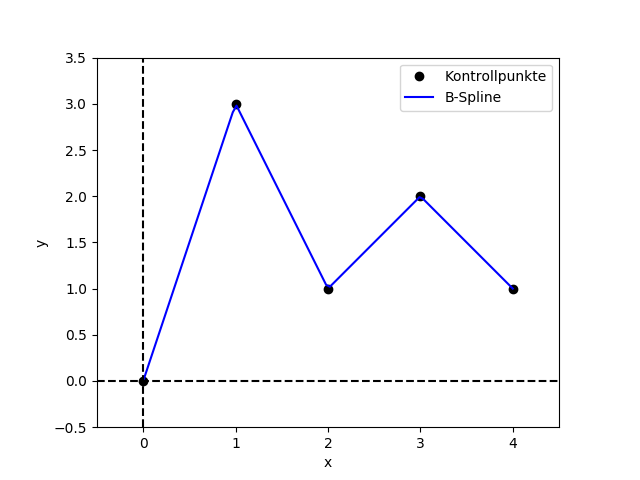
\includegraphics[width=\textwidth, keepaspectratio]{splines}
  \end{figure}
\end{center}
Wie man sieht, ist die Kurve zwar stetig, allerdings nicht stetig differenzierbar. Der Grund dafür ist, dass ein B-Spline $n$-ten Grades immer genau $(n-1)$-mal stetig differenzierbar ist. Da der Grad des hier verwendeten Splines $1$ ist, ist der Graph folglich nur stetig. Im Gegensatz zu einem Polynom mit Grad $1$ (also einer linearen Funktion) ist die Steigung des Splines allerdings nicht konstant, sondern besteht aus mehreren Abschnitten mit unterschiedlicher Steigung. Dies liegt daran, dass die Basisfunktionen der Kontrollpunkte des Splines lokalen Support besitzen, die Kurve also nur in ihrer näheren Umgebung beeinflussen. So hat z.B. der zweite Kontrollpunkt $P_1 = (1, 3)$ nur im Interval $x\in [0;2]$ einen Einfluss auf die Steigung.